\documentclass[xcolor=dvipsnames]{beamer}

\usepackage[utf8]{inputenc}
\definecolor{dgreen}{rgb}{0.,0.6,0.}
\definecolor{gold}{rgb}{1.,0.84,0.}

\usepackage{epsfig}
\usepackage{amssymb}
\usepackage{amsmath}
\usepackage{amsfonts}
\usepackage{mathtools}
\usepackage[outline]{contour}

\usecolortheme[named=dgreen]{structure}
 \setbeamertemplate{footline}[page number]

\title{Cooling-Aware Green Geographical Load Balancing Visualized}

% \subtitle{Research supported by NSF, Elliot Family, and Rose Hills Foundation}

\author[Hirshleifer, Wang, Liu, Wierman] % (optional, for multiple authors)
{Michael~Hirshleifer\inst{} \and Yizhen~Wang\inst{} \\ \and Zhenhua~Liu \inst{} \and Adam~ Wierman \inst{}}
\institute[Caltech]
{
  \inst{}%
  California Institute of Technology \\
  1200 E California Blvd \\
   Pasadena, CA 91106 \\
}
%\subject{@@@@}


% TOC at start of each section
\AtBeginSection[]
{
  \begin{frame}
    \frametitle{Table of Contents}
    \tableofcontents[currentsection]
  \end{frame}
}

\newcommand{\carbondioxide}{\ensuremath{\mathrm{CO}_2}}
\newcommand{\eqdef}{\ensuremath{\overset{\mathrm{def}}{=}}}

\date{2012-10-20}

\begin{document}

\frame{\titlepage}

\begin{frame}{Acknowledgements}
	\begin{block}{}
		We are deeply grateful to:
		
		\begin{itemize}
			\item Professor Adam Wierman for insightful and patient guidance.
			\item The NSF, Elliot family, and Rose Hills Foundation for financial support.
		\end{itemize}
		
	\end{block}
\end{frame}


\begin{frame}
\frametitle{Outline}
\tableofcontents[part=1,pausesections]
\end{frame}

\section{Introduction}

\begin{frame}
\frametitle{Motivation}
\begin{block}
{Vast, high-growth energy use by data centers.}
The Green Data Center Market Will Grow from \$17.6 Billion to \$45 Billion by 2016, Forecasts Pike Research, WSJ September 14, 2012, 5:00 a.m. ET  

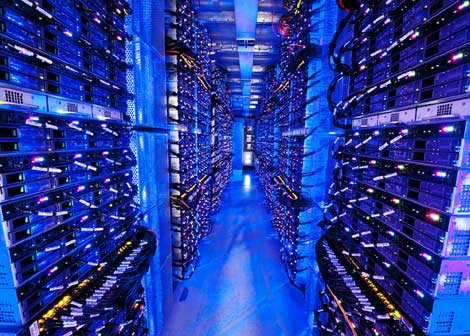
\includegraphics[scale = 0.6]{datacenter.jpg}

\end{block}
\end{frame}
%
%
\begin{frame}
\frametitle{Motivation, contd.}
\begin{block}
{How can we make them `green'?}

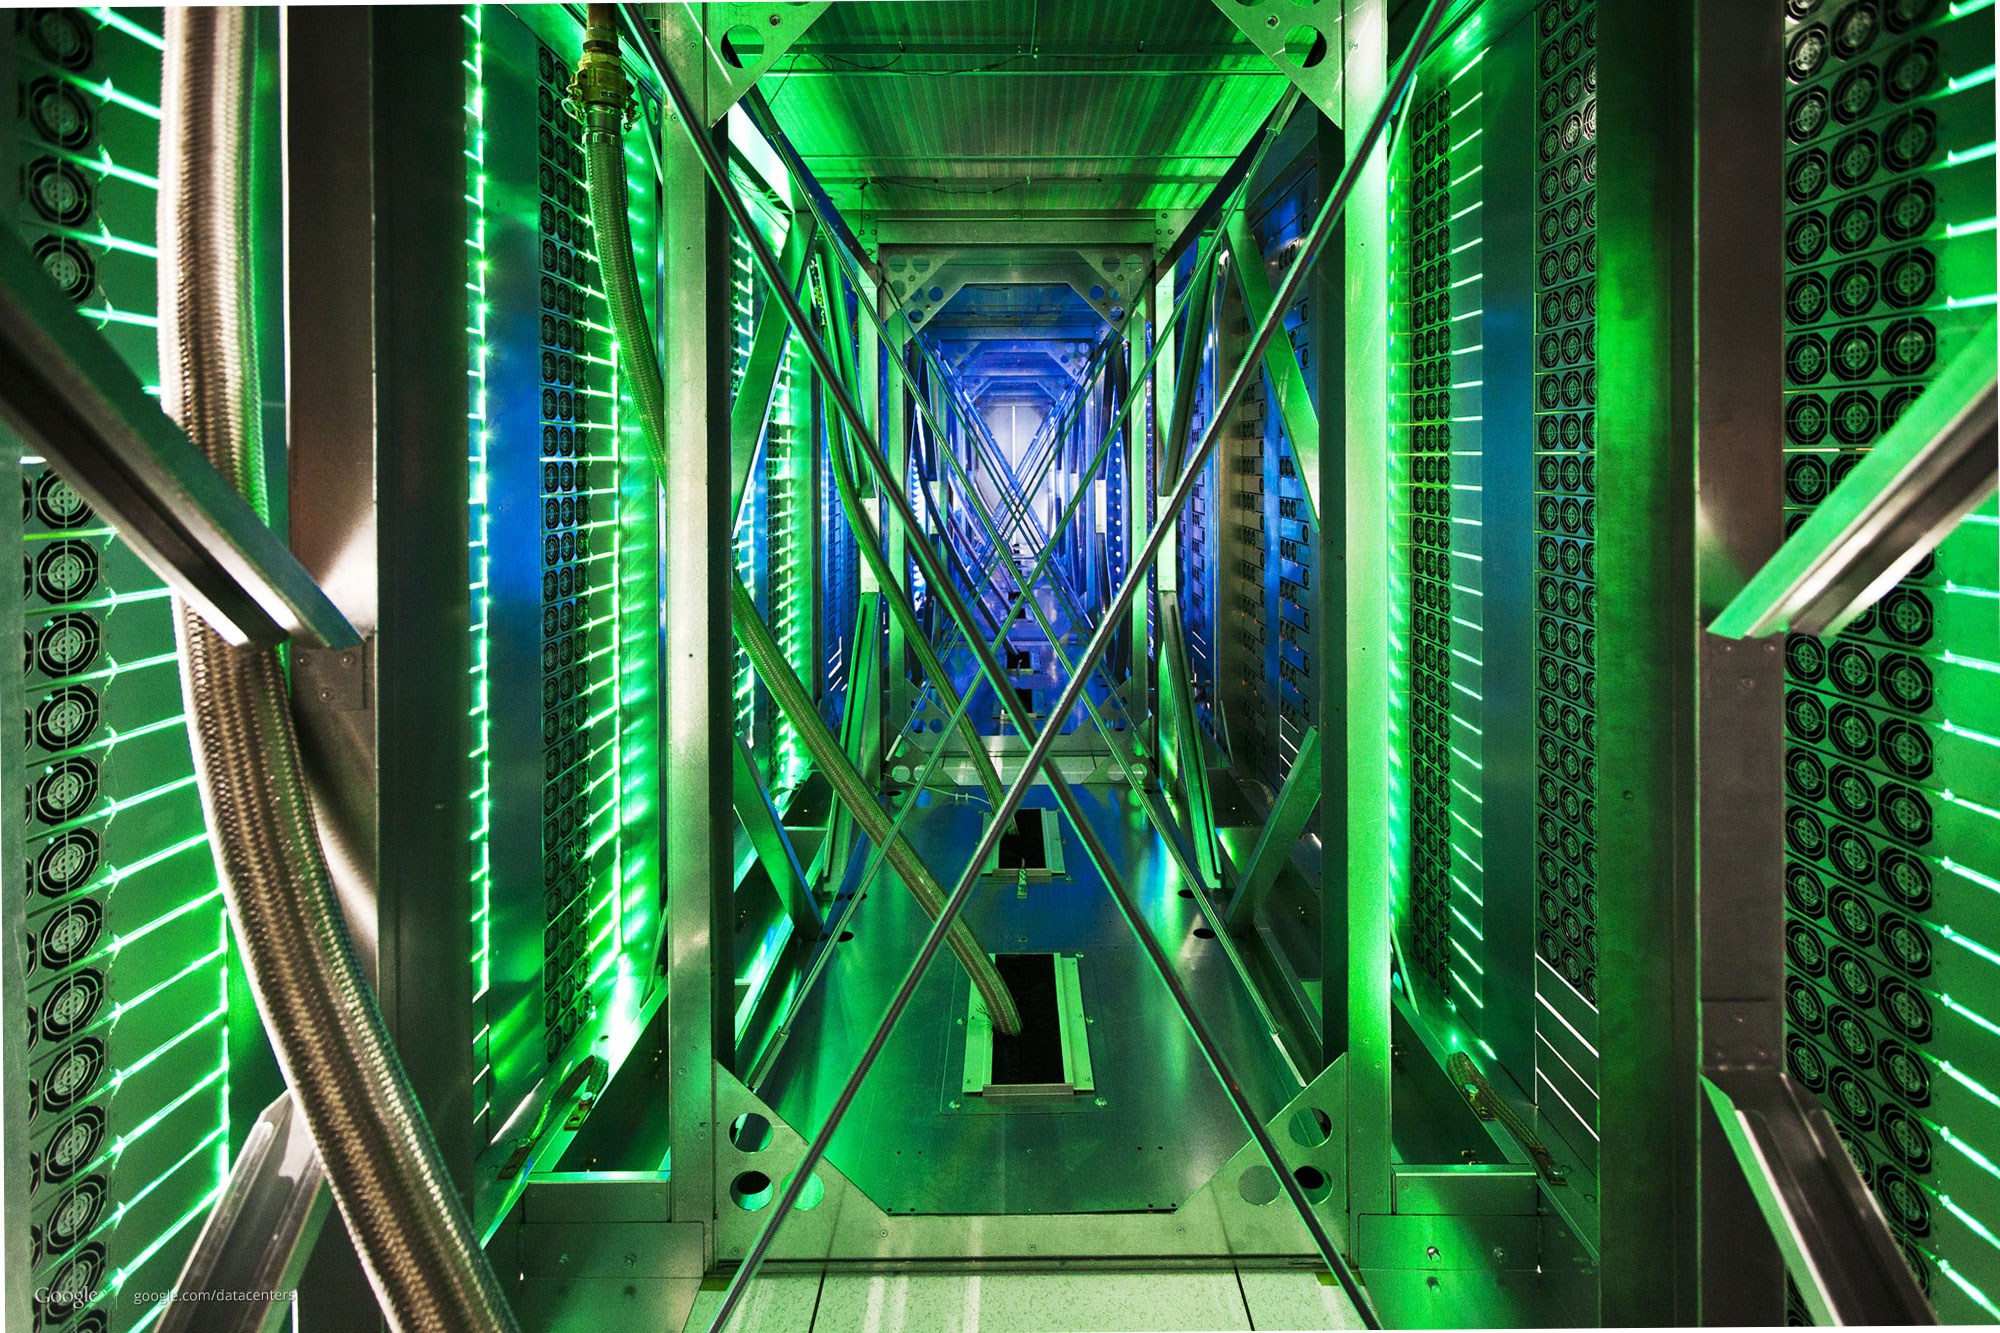
\includegraphics[scale = 0.15]{green.jpg}

\end{block}
\end{frame}
%

\begin{frame}{Motivation, contd.}
	\begin{block}{DCs use a \emph{lot} of power} 
		Substantial fraction of world non-green energy production.
		\begin{itemize}
			\item {Expensive}
			\item {Dirty (brown energy)}
		\end{itemize}	
	\end{block}

	\begin{block}{DC servers' energy demand} \vspace{-1mm}
		\begin{itemize}
		          \item{To operate and \textbf{\textcolor{blue}{cool}}}
			\item{Variable}
				\begin{itemize} 
					\item {Over time (e.g. cooling more costly in summer)}  %\cite{datacenter} 	
					\item{Cooling costs vary geographically.}
		 		\end{itemize}				
			\item{Some DCs make use of green energy (solar, wind).}
		\end{itemize}
 	\end{block}
\end{frame}

\begin{frame}{Motivation @@@@}
	\begin{block}{Use renewable energy!}
		\begin{figure}
			\centering
			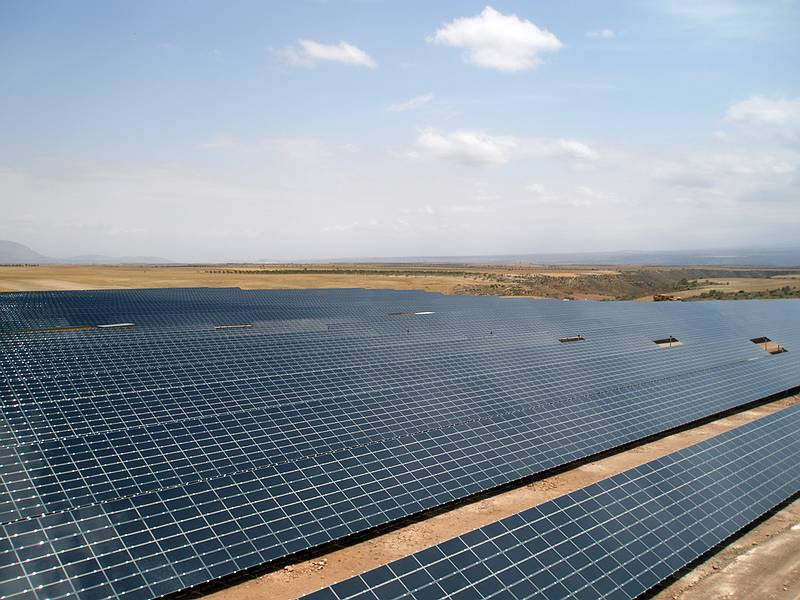
\includegraphics[height=1.5in]{PanSol2.jpg}~
			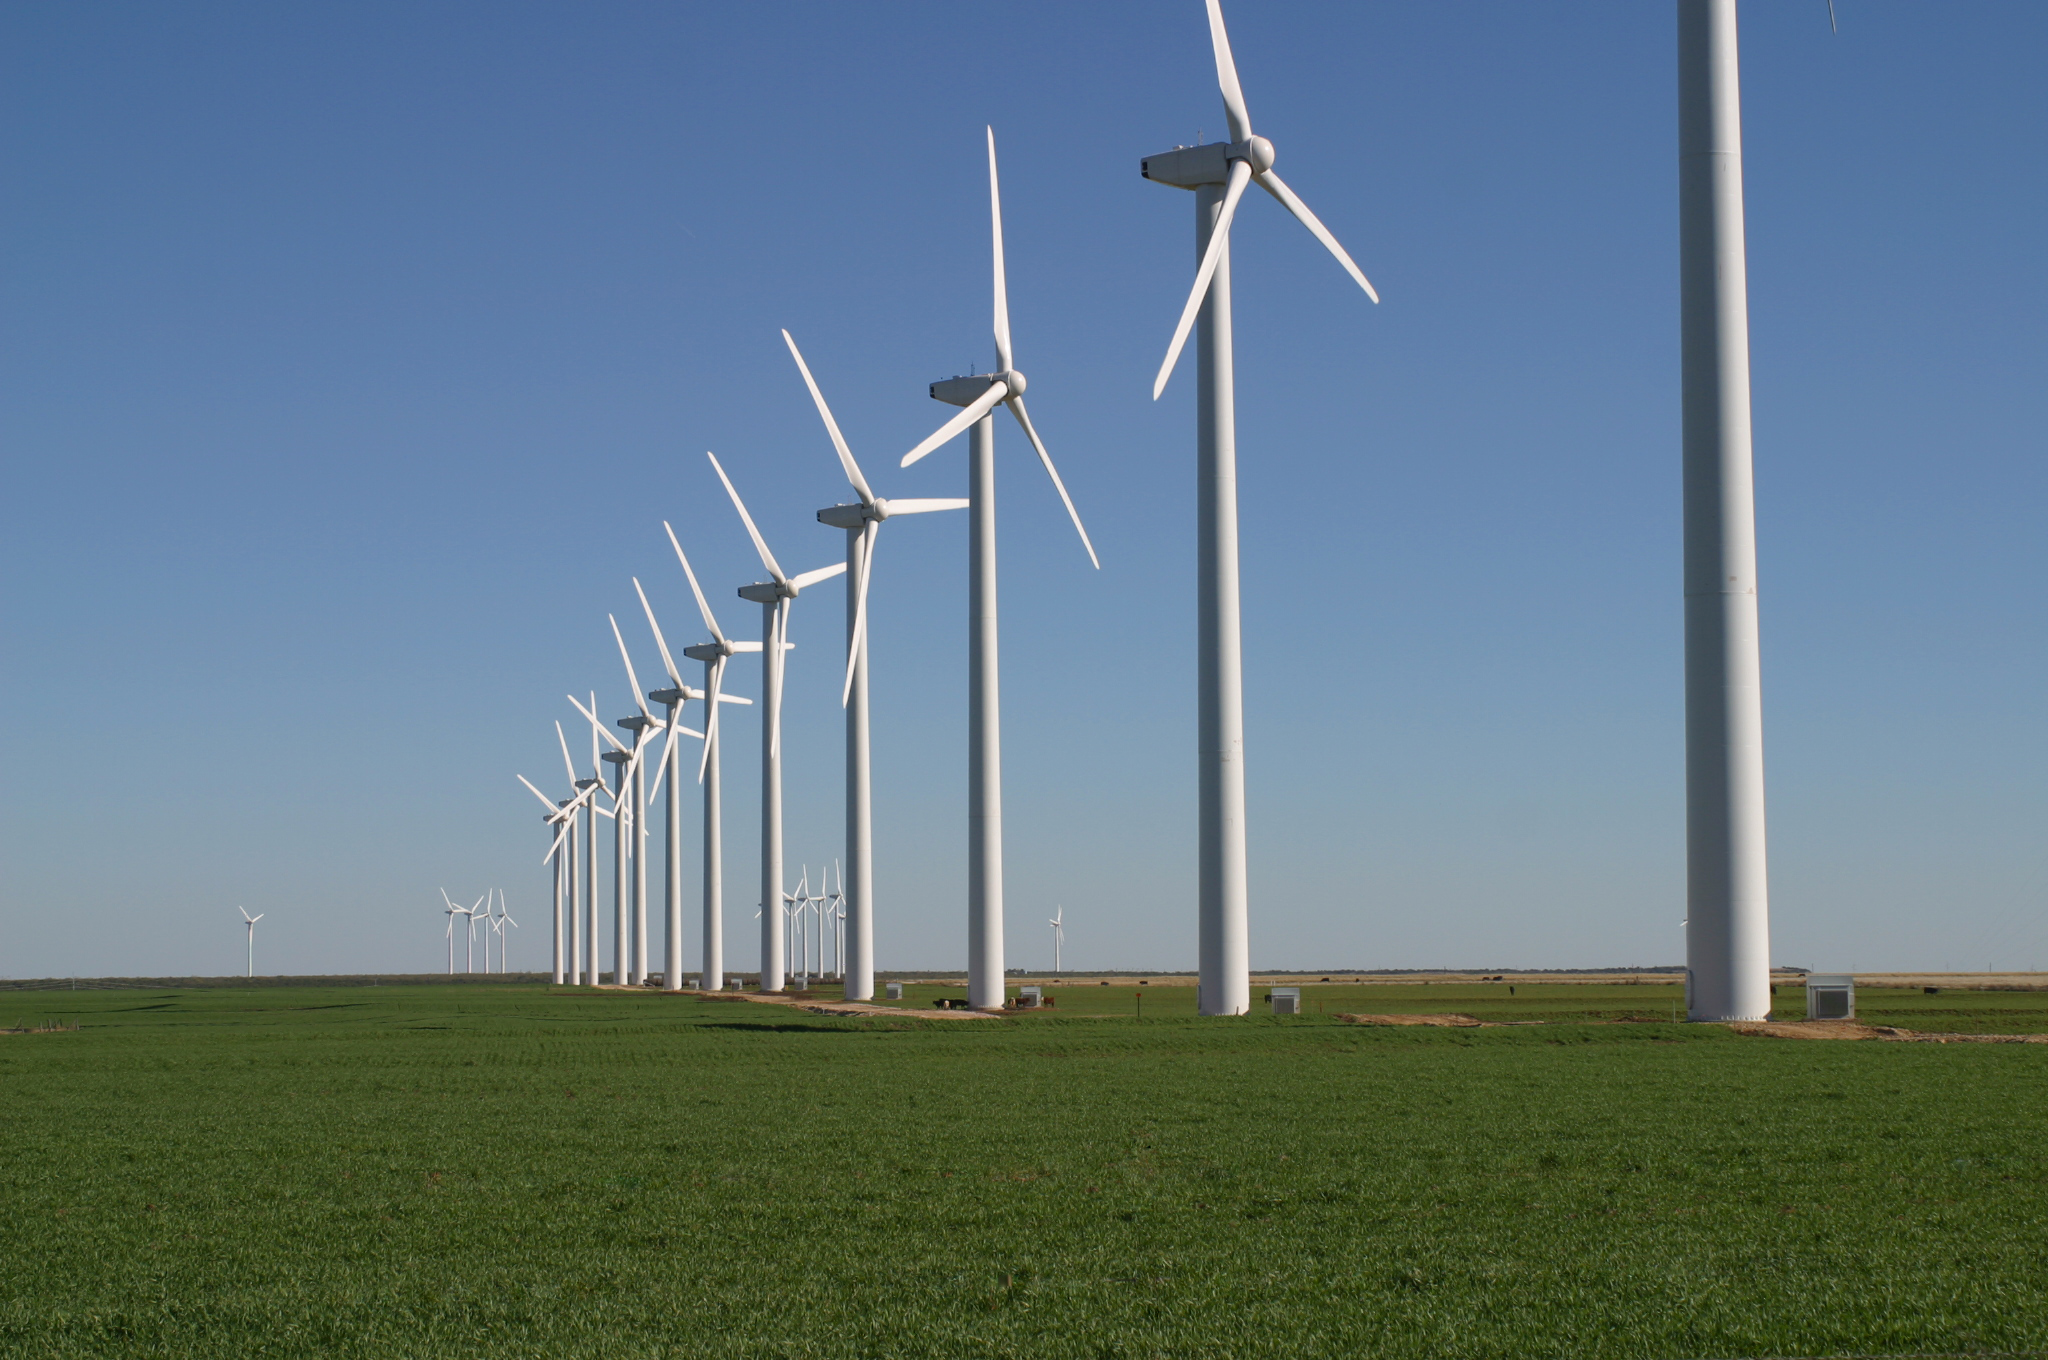
\includegraphics[height=1.5in]{GreenMountainWindFarm_Fluvanna_2004.jpg}
			\caption{Solar and wind power}
		\end{figure}
	\end{block}
\end{frame}


\begin{frame}{Motivation, contd.}

	\begin{block}{Problem: Green energy highly variable} 
		\begin{itemize}
			 \item{Time of day, cloud cover, wind speed.}
			 \item{Does not match user demand. }
			\item{Very expensive to store.}
		\end{itemize}
		Must still buy brown energy off grid \\ $\Rightarrow$ expensive; pollutes.
	\end{block}
\end{frame}

\begin{frame}{Our approach: Geographical Load Balancing}
	% Notice that in this illustration, user in OK is a bit closer to IL dc, so we route there.
	\begin{figure}
		\caption{\textbf{\textcolor{brown}{Traditional routing}}: route request to nearest DC, which minimizes latency}
		\centering
		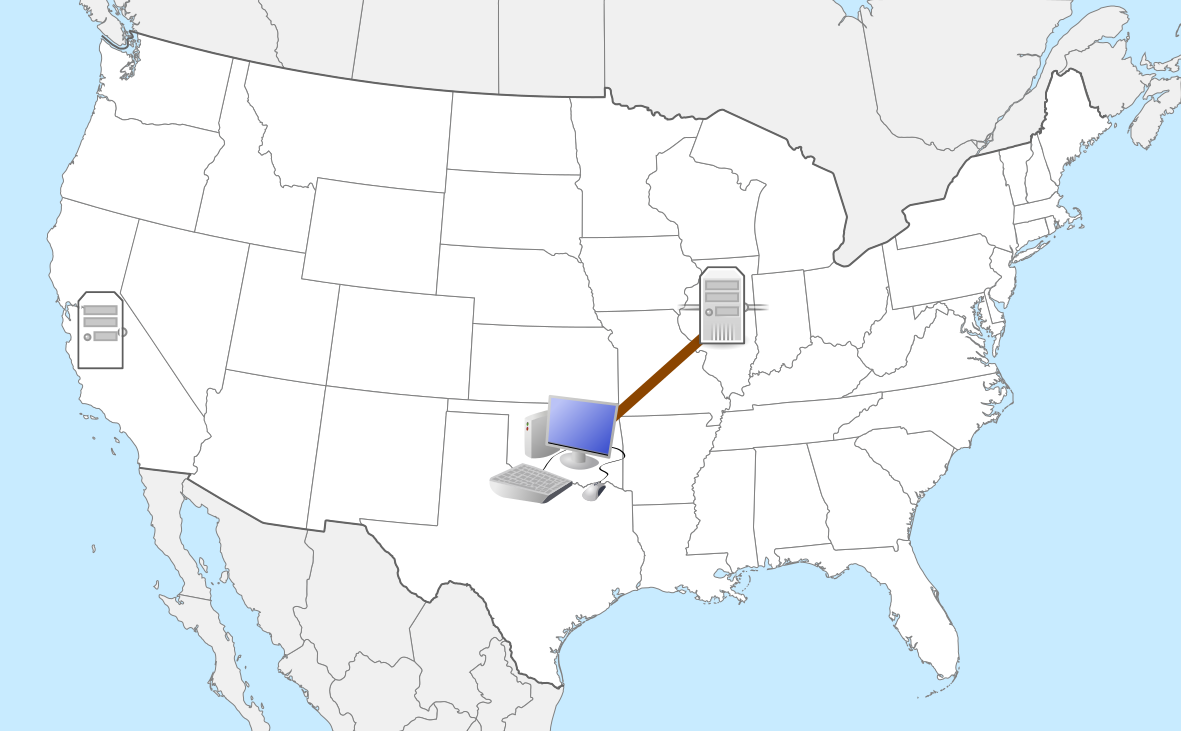
\epsfig{file=svg/nearestrouting.pdf, height=2.3in}
	\end{figure}
\end{frame}
\begin{frame}{Our approach: Geographical Load Balancing}
	% Created by Prof. Wierman's group
	% Now, it's sunny at the CA data center but cloudy at the one in IL. So route to CA, where solar power is available.
	% GLB routes requests from a population center to a data center by trading off latency with green energy use.
	% It's a good deal if Google can halve their grid energy usage for a few milliseconds more latency per Google search.
	% Balances advantage of green energy vs. cost of higher latency
	\begin{figure}
		\caption{\textbf{\textcolor{dgreen}{GLB}} (Liu et al., 2011): prefer routing to DCs that currently have renewables available}
		\centering
		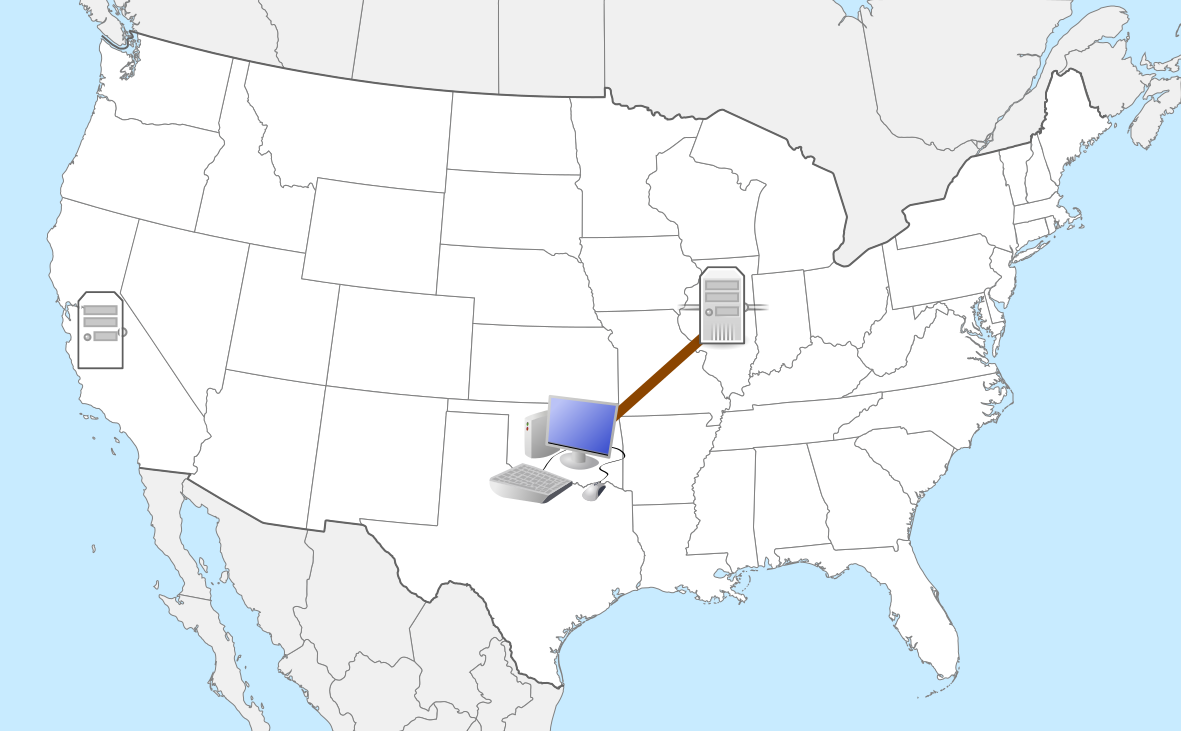
\epsfig{file=svg/nearestrouting.pdf, height=2.3in}
	\end{figure}
\end{frame}

\begin{frame}{Summary of our project}

	\begin{block}{Research goal}  
	Develop software to show how geographical load balancing (GLB) improves data center (DC) efficient use of renewable energy.  
	\end{block}
	
	\begin{block}{Issue} 
	Minimize DC electricity cost over time by convex optimization over real workload inputs - temp, solar, \& wind traces.
	\end{block}

	\begin{block}{Our contributions} 
	\begin{itemize}
		\item{Visualization \\ 
		Animation of 10 DCs' demand and usage of energy (grid \& renewable energy generation) in 48 contiguous U.S. states}
		\item{Test effectiveness of, and refine, routing algorithms using visualization}
		\item{Cooling-aware GLB model \\
			Uses locally available renewable energy more effectively \\
			Reduces electricity grid usage despite weather shifts\\
			Potentially uses renewables almost exclusively}
	\end{itemize} 
	\end{block}

\end{frame}

\begin{frame}{The cooling-aware GLB model}

		\begin{itemize}
			\item{Introduces cooling costs into GLB algorithm}
			\begin{itemize}
				\item Better-informed decisions  
			\end{itemize}
			\item{Use actual data center workload, weather, renewable energy (wind, solar) availability and grid electricity prices}
			\begin{itemize}
				\item {10 Data Center locations serving population centers in 48 contiguous U.S. states}		
			\end{itemize}
			\item{Numerically compute the optimal solution.}
			\begin{itemize}
				\item Determine economic, environmental impact
			\end{itemize}
			\item{Implement visualization of simulation solution \\
				\begin{enumerate}
					\item{Easier to see what each optimization algorithm is doing.}
					\item{Can test effectiveness of, and refine, routing algorithms.} 
					\item{Facilitate development of an implementable algorithm.}
				\end{enumerate}
				}			
			\item Compare performance using GLB vs. energy storage			
		\end{itemize}

\end{frame}

\begin{frame}{The cooling-aware GLB model, contd.}

	\begin{block}{Key insights and results}
	\begin{itemize}
		\item{Significantly lower total energy cost, \carbondioxide{} emission halved.}  %  [[Environmentally friendly
		\begin{itemize}
			\item Distributes requests to locations with cheap energy, favorable weather for cooling  % [[{Lower infrastructure investment, easier to implement }
		\end{itemize}
		\item{Cost of running data center fairly constant across seasons, weather, diurnal temp. variation}  
		\item {((( Latency ????))) performance of GLB comparable to using storage, while cost is much lower}
	\end{itemize}
	\end{block}

\end{frame}

\section{Setup}

\begin{frame}{Model setup}

Modify Liu et al.'s (2011) %\cite{adam:GLB}% 
model to include cooling costs.

\vspace{3mm}
\begin{block}{\underline{Key factors}}
\end{block}
\vspace{-2mm}
	
\begin{block}{IT Load}
\end{block}
\vspace{-2mm}

 \begin{block}{Supply of renewables at different DCs}
\end{block}
\vspace{-2mm}

\begin{block}{Storage}
\end{block}
\vspace{-2mm}

\begin{block}{Costs} 
	\begin{itemize}
		\item Total Cost = Energy Cost + Propagation \& Queuing Delay Costs + Switch Cost
		\item {\bf \textcolor{blue}{New: Cooling costs}}
		\item 2 Cooling options - Air, Chilled-Water 
	\end{itemize}
\end{block}

\end{frame}

\begin{frame}{Assumptions}


	\begin{block}{IT Load $L$ in each state}
 	\begin{itemize}
		\item 	Obtain base load from real-world traces (HP Labs).
		\item 	Scale by state population. 
		\item 	Shift by time zone.
	\end{itemize}
	\end{block}
\vspace{-3mm}
	\begin{block}{Data centers}
			\begin{itemize}
				\item        1 Google data center in each of 10 states. % limit = 2 $\times$ peak load at $i$  \vspace{1mm} 
				\item 	Capacity limited by finite \# servers in each DC.
			\end{itemize}
	\end{block}
\vspace{-3mm}
	\begin{block}{Renewable availability} 
	\begin{itemize}
		\item 	DCs use combination of green \& brown energy sources.
			\begin{itemize}
				\item  Use avg mix of 80\% of wind and 20\% solar (Liu et al. 2011). % \cite{adam:GLB}.
			\end{itemize}
		\item  Proportional to wind speed \& solar irradiance; from http://wind.nrel.gov/.  %\cite{renew1} \cite{renew2}. 
		\item Fluctuates with season, sunrise/sunset time
		\item Capacity = $c \times$ national aggregate demand under full load
		\end{itemize}
	\end{block}
\end{frame}

\begin{frame}{Cost factors}
	\begin{description}
		\item[Optimization problem:] Choose routing plan and \# active servers to minimize total cost (= delay cost + switching cost + energy cost).
	\end{description}
	% Use \only to collapse sections so that everything fits.
	\begin{block}{Delay cost}\only<1>{
		Business cost of request latency (distance traveled, queuing delay at DC)
		\begin{itemize} \item Calculated using a sharing queue model. \end{itemize}
		% Total load $\lambda_i(t)=\sum_j \lambda_{ij}(t)$ distributed evenly across $x_i(t)$ homogeneous servers of service rate \mbox{$\mu_i$ = $0.1 /
		%  \mathrm{ms}$}.
	}\end{block}
	\vspace{-3mm}
	\begin{block}{Switching cost}\only<1>{
		Delay, wear-and-tear cost from powering servers on/off. %DC workload updated every 10 mins. 
		% Switching cost weight $\beta = 6$.$$\beta \cdot (x_i(t+1) - x_i(t))^+$$
	}\end{block}
	\vspace{-3mm}
	\begin{block}{Energy cost}\only<2>{
		Cost of the energy used to power the DC.
		\begin{itemize}
			\item Demand
			\begin{description}
				\item[\textcolor{yellow}{\contour{black}{IT cost}}] running active servers (CPU, disk, ...)
				\item[\textcolor{blue}{cooling}]
			\end{description}
			\item Supply
			\begin{description}
				\item[\textcolor{green}{\contour{black}{renewable}}] free
				\item[\textcolor{brown}{grid}] depends on market price in each state, amount used
			\end{description}
		\end{itemize}
		% \begin{equation}
		%p_i \cdot (l(x_i(t)) + c(x_i(t)) - r_i(t))^+
		%\end{equation}
		%$p_i$ = electricity price, 
		%$x_i(t)$ = \#active servers in time interval $t$,
		%$l(x_i(t))$ = linear function of energy consumption, %of active servers or IT demand in time interval 
		%$c(x_i(t))$ = energy usage for cooling, $r_i(t)$ = renewable energy availability, 
		%$p_i$  = constant real statistic for each state. 
	}\end{block}
	\vspace{-3mm}
	\pause % Make Beamer generate 2 slides
\end{frame}

\begin{frame}{\textcolor{blue}{Cooling costs}}

  
%	Minimize energy consumption to maintain DC at $T = 25^{\circ}\textrm{C}$. 
%	\#active servers $x = x_a + x_c$  where a=air-cooled, c=water chilled. \vspace{1mm} 
%	Find best division between $x_a$ and $x_c$.
%	\begin{block}{Air-cooling energy consumption} \vspace{-3mm}

% ********** Fix in paper ******
%	\begin{equation}
%          c_a(x) = k \cdot (x_a)^3, 0 \leq x_a \leq \bar{x}, k > 0
% 	\end{equation}
% ************
% $k$ $\propto$ temperature gradient between the inside and outside air. 

%$\bar{x}$ = maximum \#servers cooled by air cooling alone. 

%$\bar{x}$ $\propto$ temperature gradient, maximum air flow rate. 

\begin{itemize}
	\item Part of energy cost (demand)
	\item Air cooling cheaper when outside air is cold
	\item Water cooling (relatively) cheaper when outside air hot.
	% Set air flow rate to level that can air cool DC entirely at full workload when outside temperature is lower than   $T - 20^{\circ}\mathrm{C}$. 
	\item Cost of chilled-water cooling proportional to processing load (active servers) cooled with water.
	\item Air cooling cost rises nonlinearly with processing load.
	\item So DC chooses amount of air- vs. water-cooling, as a function of total processing load, to minimize cost (convex optimization).
\end{itemize}

% *********** Fix in paper ***********
% \begin{equation}
% c_c(x) = \gamma \cdot x_c
% \end{equation}
% Here $\gamma = 0.17$, meaning that the chiller takes 0.17kW/h electricity to cool the heat caused by 1kw/h of IT demand.
% For notational convenience, define
% \begin{equation}
%	x^+ \eqdef \min(0, x)
% \end{equation}
% to be $x_c$ **** constrained *** to be positive.

%\begin{block}{Optimal cooling portfolio}
%\begin{equation}
%c(x) = \min_{x_c \in [0,x]} \gamma \cdot (x-x_a)^+ + k(x_a)^3
%\end{equation}
%which yields
%$$
%c(x) = \left\{ \begin{array}{ll}
%	k \cdot x^3 & \mbox{if $x \geq x_s$}\\
%	k \cdot x_s^3 + \gamma \cdot (x-x_s) & \mbox{otherwise}\end{array} \right.
%$$
%where $x_s = \min \left(\sqrt{\gamma/3k}, \bar{x}\right)$ is the threshold for when chiller cooling is necessary.
%\end{block}


%To explore seasonality on cooling model performance
% Hourly temperature data from Week 1 January 2012 from \cite{temp} and Week 1 July 2012. 
\end{frame}

\begin{frame}{Minimize total costs using convex optimization}

\begin{align*}
&\underset{\bf{x}(t), \bf{\lambda}(t)}{\text{minimize}} & \hspace{0.5em}
	& \mathrlap{\sum_{i \in \mathcal{N}} p_i \cdot (l(x_i(t)) + c(x_i(t)) - r_i(t) - e_i(t))^+} \\
	&&& \mathrlap{{} + \sum_{j \in \mathcal{J}}\sum_{i \in \mathcal{N}} \lambda_{ij}(t)\left(\frac{1}{\mu_i - \lambda_i(t)/x_i(t)} + d_{ij}\right)} \\
	&&& \mathrlap{{} + \beta \cdot (x_i(t+1) - x_i(t))^+} \\
\\
&\text{\textcolor{blue}{subject to}}
	&& \sum_{i\in \mathcal{N}}\lambda_{ij}(t) = L_j(t), &\forall j\in J \\
	&&& \lambda_{ij} \geq 0, & \forall i\in N, j\in J \\
	&&& 0 \leq x_i(t) \leq X_i, & \forall i \in N \\
	&&& \lambda_i(t) \leq x_i(t) \cdot \mu_i & \forall i \in N \\
	&&& 0 \leq es_i(t) \leq ES_i & \forall i \in N \\
	&&& e_i(t) = es_i(t) - es_i(t+1) & \forall i \in N
\end{align*}

\end{frame}

\begin{frame}{Minimize total costs using convex optimization}

\begin{align*}
&\underset{\bf{x}(t), \bf{\lambda}(t)}{\text{minimize}} & \hspace{0.5em}
	& \overbrace{ \sum_{i \in \mathcal{N}} p_i \cdot (l(x_i(t)) + c(x_i(t)) - r_i(t) - e_i(t))^+ }^{\text{\textbf{\textcolor{red}{energy cost}}}} \\
	&&& {} + \overbrace{ \sum_{j \in \mathcal{J}}\sum_{i \in \mathcal{N}} \lambda_{ij}(t)\left(\frac{1}{\mu_i - \lambda_i(t)/x_i(t)} + d_{ij}\right) }^{\text{\textbf{\textcolor{red}{delay cost}}}}  \\
	&&& {} + \overbrace{ \beta \cdot (x_i(t+1) - x_i(t))^+ }^{\text{\textbf{\textcolor{red}{switching cost}}}}
\end{align*}
\vspace{-2mm}

 %\fcolorbox{red}{white}{*****}
%Min (\#servers, routing plan)  [Grid costs + 
%\end{frame}
%\begin{frame}{}

	\begin{block}{\textcolor{blue}{Boundary conditions model real-world constraints:}}
	\begin{itemize}
	\item
	GLB system processes all requests. Each DC gets $>0$ work.
	\item
	Each DC has finite server capacity. %cannot process requests $>$ computational capacity; server capacity finite.
	\item
	Each DC's energy storage capacity bounded.
	\end{itemize}
	\end{block}
\end{frame}

\section{Visualization}
\begin{frame}{Motivation for Visualization}
Numerical simulation result is very large time series describing routing plans and data center activity. \\
\vspace{2mm}
Hard to interpret large quantity of data in matrix form. \\
\vspace{2mm}
Visualization:  
	\begin{itemize}
	\item Key characteristics of the optimal solution salient.
	\item Acts as simple check for validity of solution
	\item An obvious way to spot abnormal behaviors in the output.
	\end{itemize}
\end{frame}
\begin{frame}{Technical description}
 	\begin{block}{Scalable Vector Graphics (SVG) format}
	High-quality XML-based vector graphics format supports fluid animations displaying time-series data. \\ 
	Animation can be embedded into a web page.
	\begin{block}{Wrapper XHTML web page} 
	Implemented using Javascript \\	
	User-friendly, can control animation (play, pause, or seek) using web interface \\
	Possible enhancements could include zooming, panning, and showing/hiding types of map elements.
	\begin{block}{Both components work in the Chromium web browser and pass the W3C validators}
	\end{block}
	\end{block}
	\end{block}
\end{frame}
\begin{frame}{Technical description, contd.}
	\begin{block}{Back-end script generating SVG map from input data}
	Written in Scala programming language. \\
	Script reads in and displays DC center locations, client (request source) locations, real solar- and wind-generation traces. \\
	Routings optimized using various algorithms (from Matlab optimization outputs). \\
	Raw input data in CSV format.\\
	Matlab outputs exported to NetCDF format for reading into Scala.
	\end{block}

\end{frame}

\begin{frame}{Data center visualization}

\begin{figure}
\centering
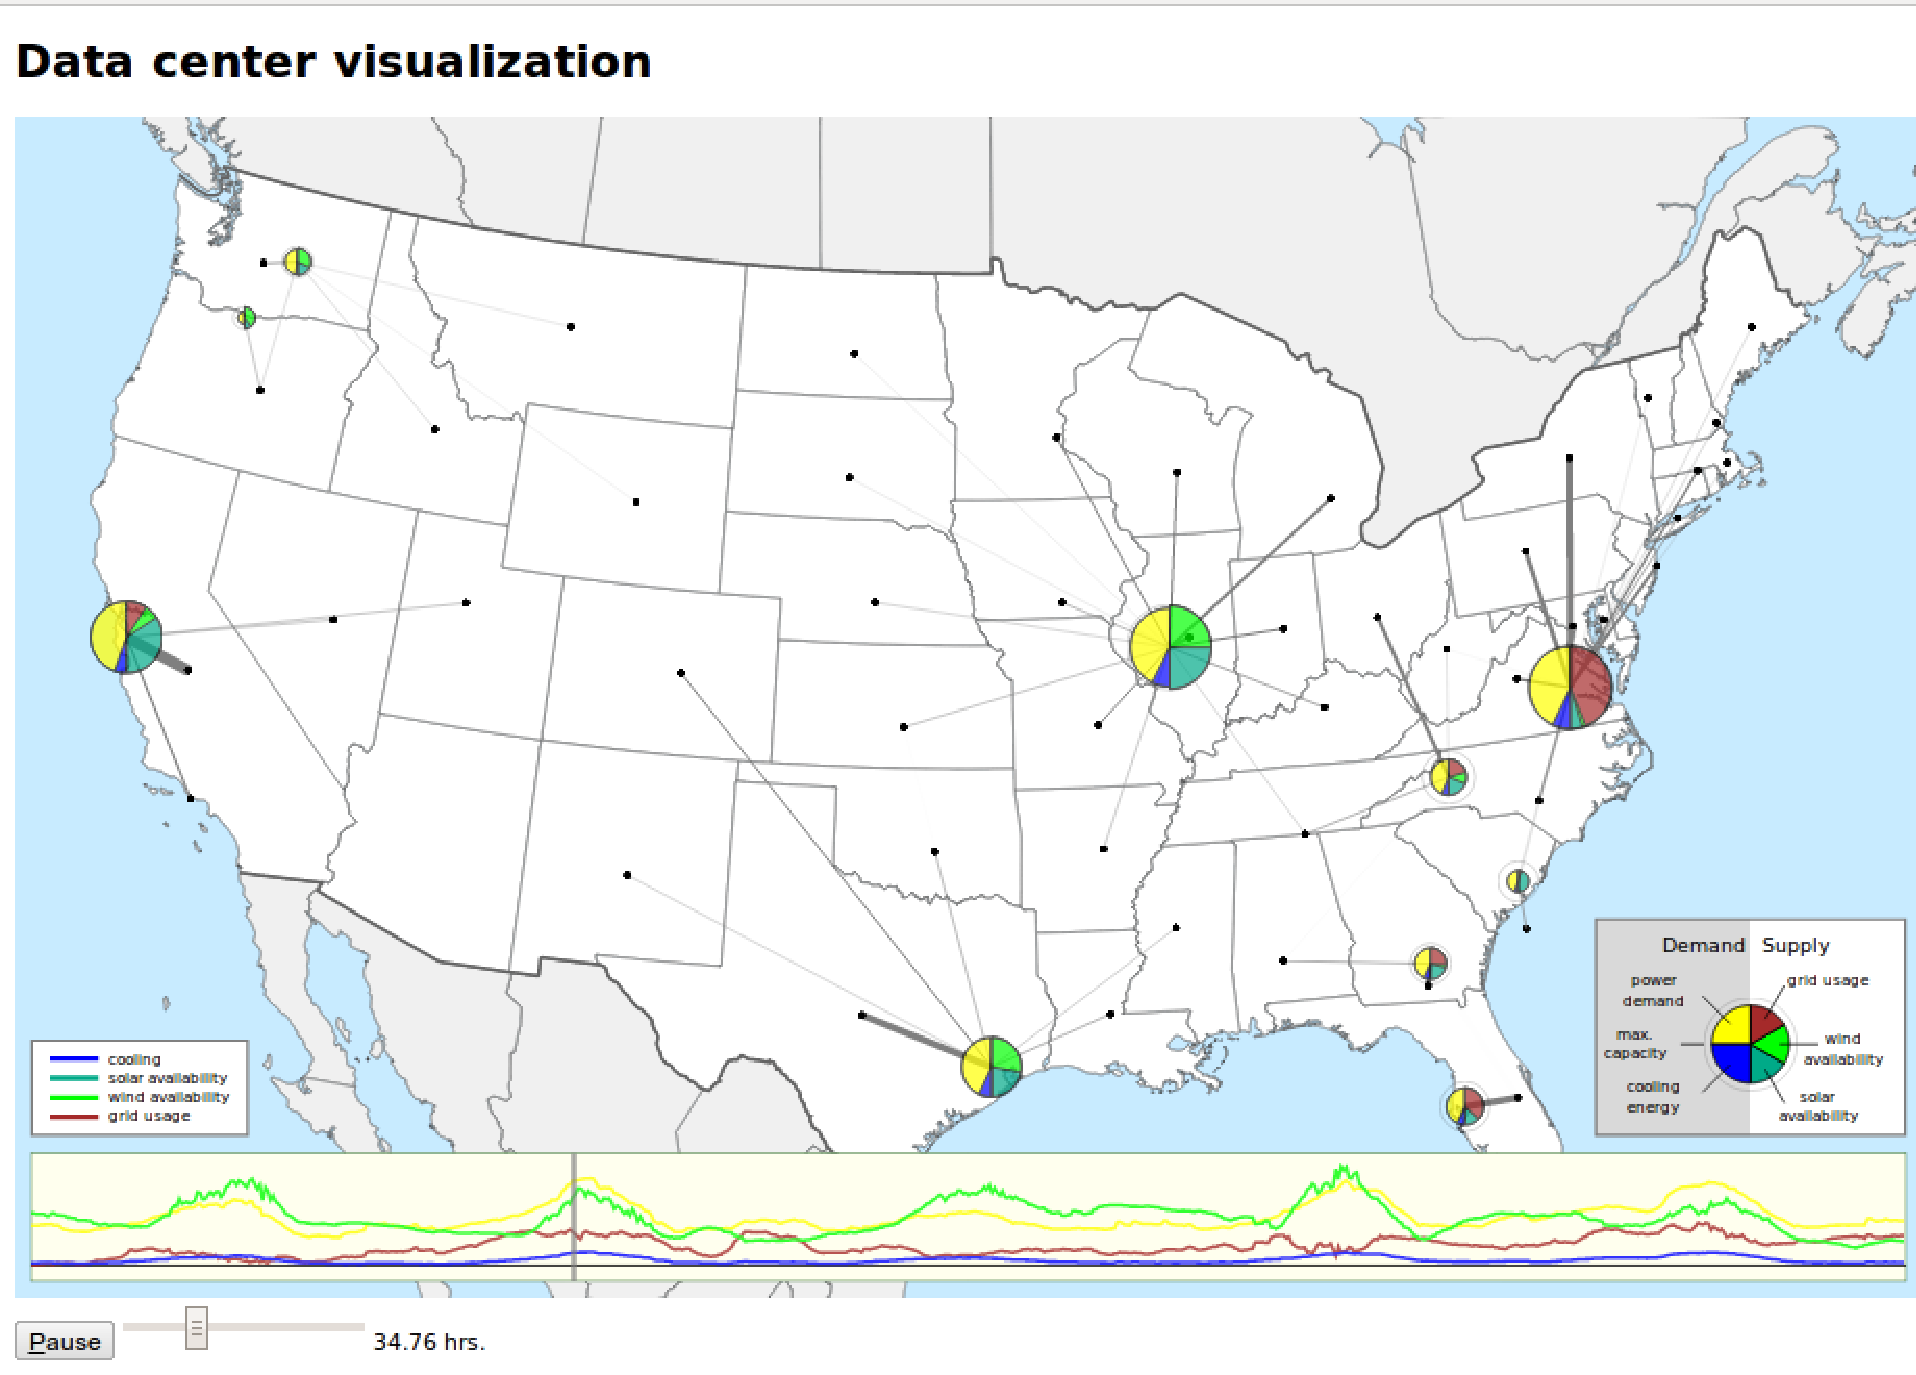
\epsfig{file=visualization-bmp.pdf, height=3in, width=4.5in}
\caption{Screenshot of the visualization, running in the Chromium web browser.}
\end{figure}

\end{frame}

\begin{frame}{Graphical representation details, Speaker Notes}

	\begin{block}{Background map of the 48 contiguous United States}
		\begin{itemize} 
		%Obtained from Wikimedia Commons. \\
	\item 	Points on map correspond to real-world $(latitude, longitude)$ coordinates according to a mathematical transformation specified with map. 
	\item 	Allows drawing physical locations at correct positions on map.
		\end{itemize}
	\end{block}
\vspace{-3mm}
	\begin{block}{Visualization's three components}
	Animation of dynamic status of the GLB system. \\
	Line plot of aggregate statistics of energy supply and demand. \\  
	Progress bar allows progress scroll and control.
	\end{block}
\end{frame}

\begin{frame}{Graphical representation details, Speaker notes contd.}
	\begin{block}{Features}
	Animation displays 10 data centers on base map of United States. \\
	Sector diagram represents each DC's status, which is animated over time. \\
	Circle's left half is DC's energy demand: 
		\begin{itemize}
		\item{\textcolor{yellow}{\contour{black}{Yellow sector = energy demand for processing the request}}}
		\item{\textcolor{blue}{Blue sector = energy demand for cooling} }
		\end{itemize}
	Circle's right half is energy supply: 
		\begin{itemize}
		\item{\textcolor{green}{\contour{black}{Light green sector = available wind energy}}}
		\item{\textcolor{dgreen}{Dark green sector = available solar energy}}
		\item{\textcolor{brown}{Brown sector = energy usage from the grid}}
		\end{itemize} 
           \end{block} 
\end{frame}

\begin{frame}{Graphical representation details, Speaker notes, contd.}

	Area of sector $\propto$ amount of energy (so radius $\propto$ to $\sqrt{}$). \\ 
	Faint circle surrounding sector diagram represents maximum energy usage when DC operates at full load. \\
	Request traffic $\lambda_{d,s}(t)$ represented by lines connecting each source $s$ and destination data center $d$. \\
	Line width linearly $\propto$ $L_s(t)$, total volume of requests from $s$. \\
	Line transparency linearly $\propto$ ${\lambda_{d,s}(t)} / {L_s(t)}$, percentage of traffic from source $s$ routed to DC.  \\
	Solid black line means all requests from $s$ are sent to $d$. \\
	Fully transparent line means no traffic routed from $s$ to $d$.
\end{frame}

\begin{frame}{Graphical representation details, Speaker notes, contd.}
	Line plot displays four aggregate statistics of interest over time: 
	\begin{itemize}
	\item{\textcolor{yellow}{\contour{black}{Yellow line = aggregate IT power}}}
	\item{\textcolor{blue}{Blue line = aggregate energy usage on cooling}}
	\item{\textcolor{green}{\contour{black}{Light green line = aggregate wind energy available}}}
	\item{\textcolor{dgreen}{Dark green line = aggregate solar energy available}.}
	\end{itemize}
	Bottom progress indicates time elapsed in animation. \\
	User can pause/resume animation and seek to desired time.
\end{frame}


\section{Testing effectiveness of results}

\begin{frame}
\frametitle{Experiment Result}
\begin{block}
{Cost saving}
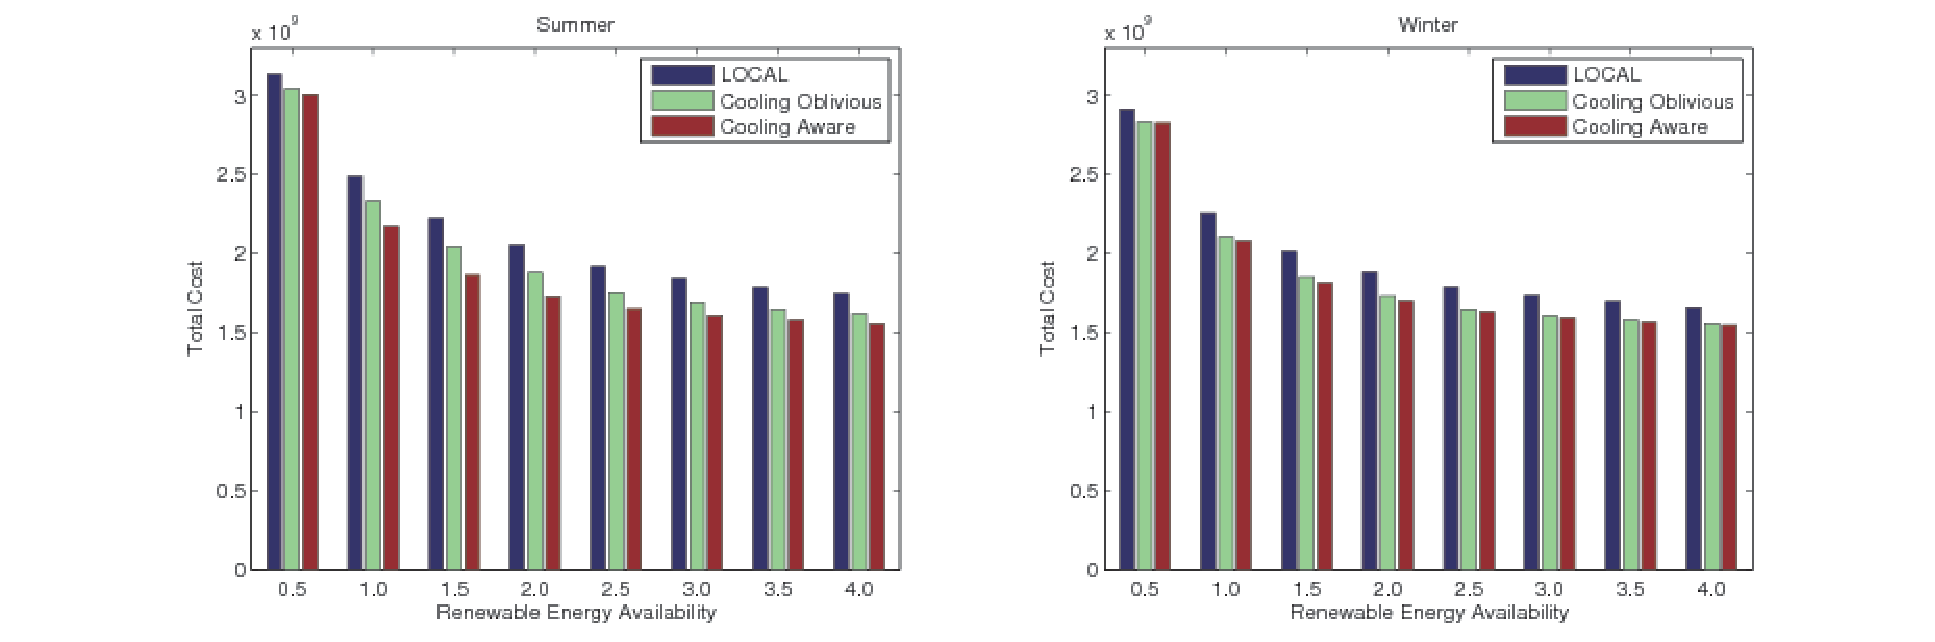
\includegraphics[scale = 0.37]{cost_comparison.pdf}
\end{block}
\end{frame}
%
%
\begin{frame}
\frametitle{Experiment Result}
\begin{block}
{Seasonality}
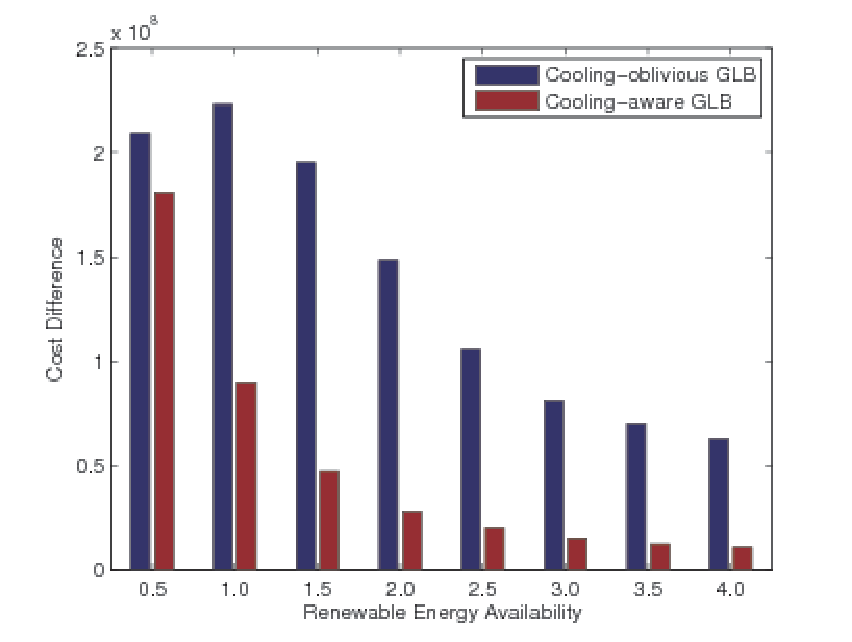
\includegraphics[scale = 0.5]{cost_diff.pdf}
\end{block}
\end{frame}
%
%
\begin{frame}
\frametitle{Experiment Result}
\begin{block}
{Carbon Emission}
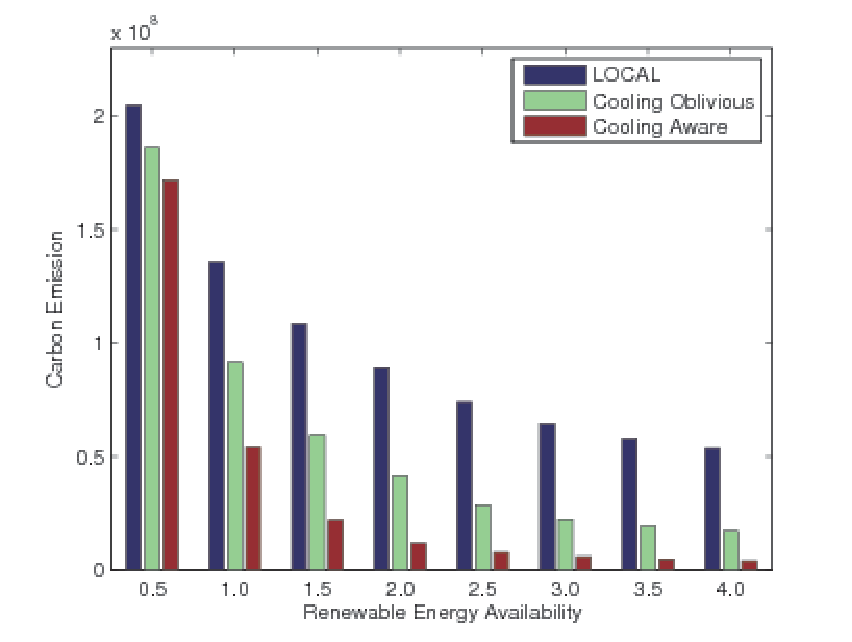
\includegraphics[scale = 0.5]{carbon_summer.pdf}
\end{block}
\end{frame}
%
%
\begin{frame}
\frametitle{Experiment Result}
\begin{block}
{vs Storage}
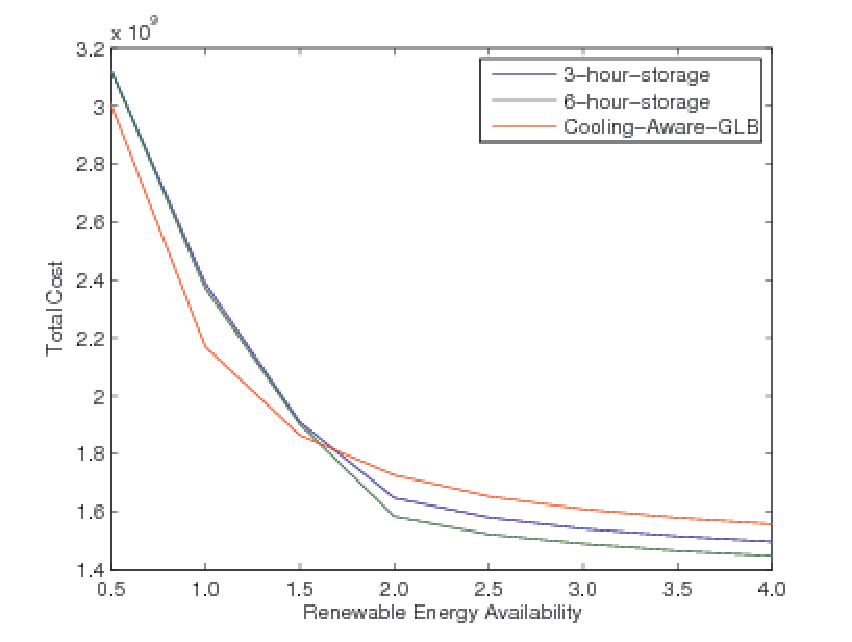
\includegraphics[scale = 0.5]{cost_storage.pdf}
\end{block}
\end{frame}
%
%
\begin{frame}
\frametitle{Experiment Result}
\begin{block}
{vs Storage}
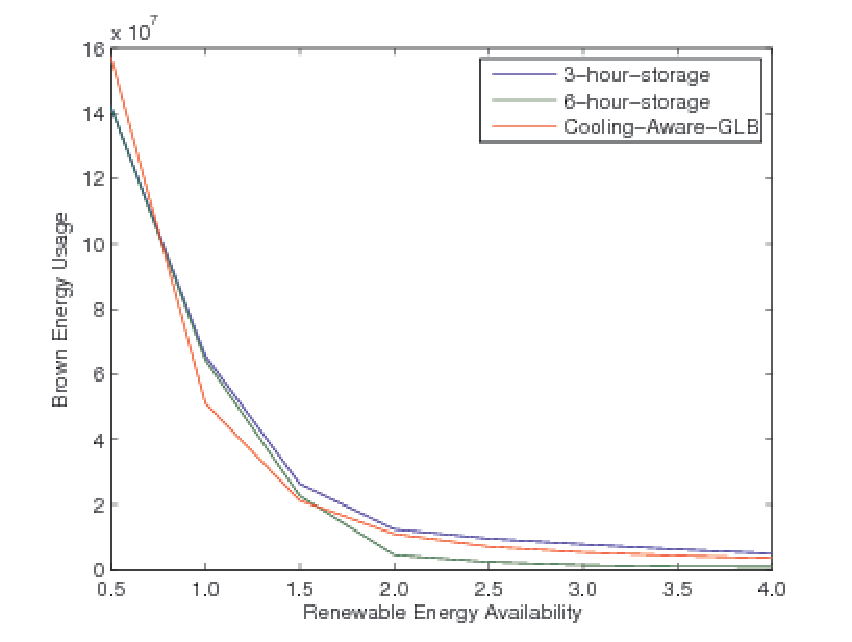
\includegraphics[scale = 0.5]{brown_storage.pdf}
\end{block}
\end{frame}
%
%
%\begin{frame}
%\frametitle{Future Work}
%\begin{block}
%{We can still improve}
%\begin{itemize}
%\item
%the online algorithm
%	\begin{itemize}
%	\item
%	involves prediction, needs to be close the optimal.
%	\end{itemize}
%\item
%dynamic pricing
%	\begin{itemize}
%	\item
%	involves changing energy price, which is the general case.
%	\end{itemize}
%\end{itemize}
%\end{block}
%\end{frame}

\begin{frame}{Future work}

Extend simulation and visualization software to:

\begin{itemize}
\item Incorporate other kinds of renewables - tailor to local renewables \& storage systems.
\item Endogenize data centers - Build new ones? 
\item Optimize timing of switching routes - currently assume algorithm switches routing at fixed time intervals. 
%Bogus? \item Optimize by relying more on wind - currently assume 80/20 wind/solar mix but almost always windy somewhere whereas night fall in large swath of US for part of day. 
\item Examine dynamic grid price.  
\item Allow DCs to sell excess renewable energy back to grid.
\end{itemize}

\end{frame}
\end{document} 



\begin{frame}{}

\begin{block}{Benchmarks to compare Cooling-aware GLB to other models.}
%To show effect of integrating cooling concerns into GLB, 
%For the two benchmark models, the cooling optimization is done after the routing scheme is determined.
%Assume 3-hr and 6-hr storage systems, no running costs for storage, finite storage capacity. 
% quantified as duration DC operates at max load entirely off stored energy (excl. cooling usage). 
\end{block}
\begin{block}{Evaluate outcomes based on (1) the total cost, (2) grid (brown) energy usage, (3) \carbondioxide{} emissions.}
\end{block}
\end{frame}

%\begin{frame}{}
%	\begin{figure}
%	\centering
%	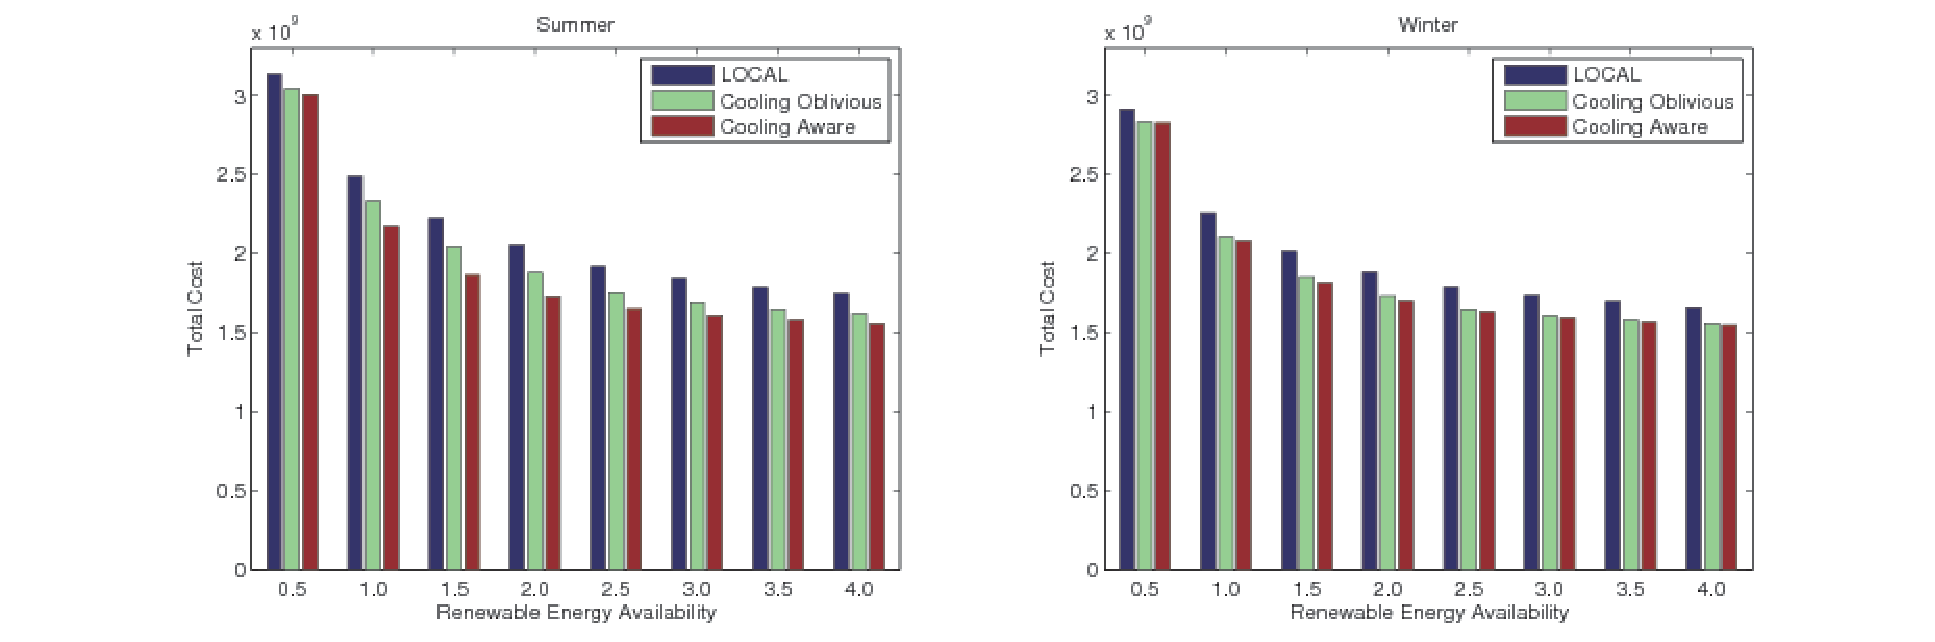
\epsfig{file=cost_comparison.pdf, height=1.8in, width=7in}
%	\caption{Comparison of optimal costs of Cooling-aware GLB, Cooling-oblivious GLB and LOCAL, with varying renewable energy availability.}
%	\end{figure}
%\end{frame}

\begin{frame}{}
	\begin{figure}
	\centering
	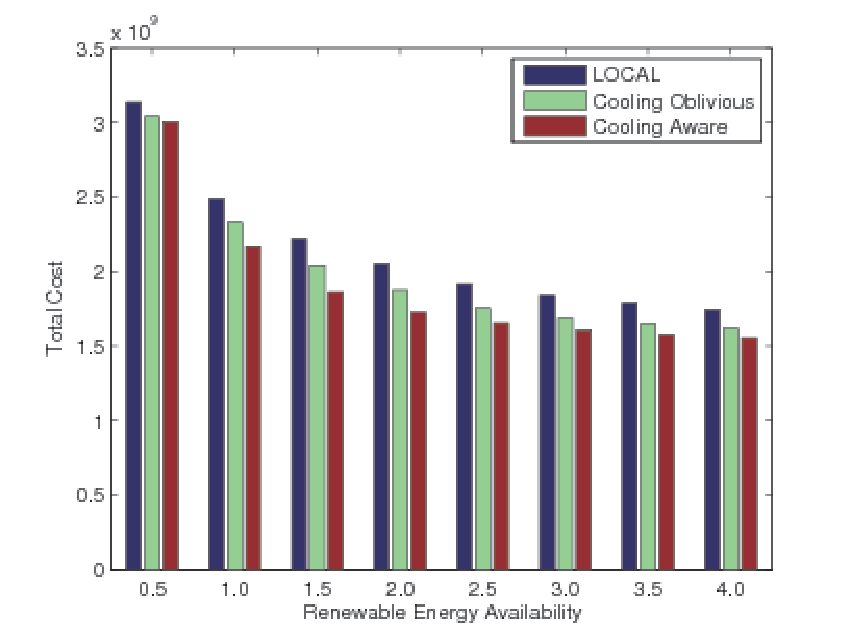
\epsfig{file=cost_summer.pdf, height=1.8in, width=4.2in}
	\caption{Summer optimized costs of Cooling-aware GLB, Cooling-oblivious GLB and LOCAL, with varying renewable energy availability.}
	\end{figure}
\end{frame}

\begin{frame}{}
	\begin{figure}
	\centering
	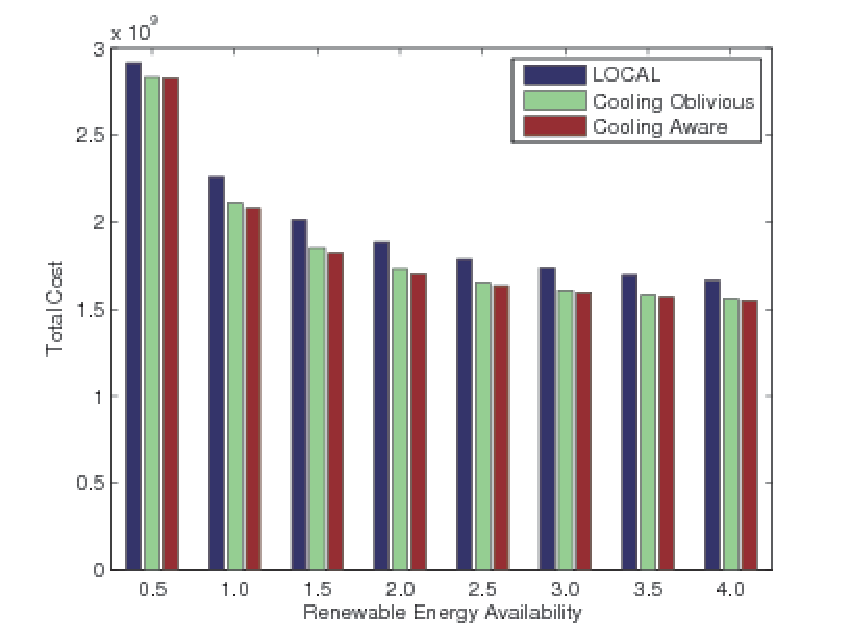
\epsfig{file=cost_winter.pdf, height=1.8in, width=4.2in}
	\caption{Winter optimized costs of Cooling-aware GLB, Cooling-oblivious GLB and LOCAL, with varying renewable energy availability.}
	\end{figure}
\end{frame}



\end{document}



\begin{frame}{Environmental impact - \carbondioxide{} savings}

\begin{figure}
\centering
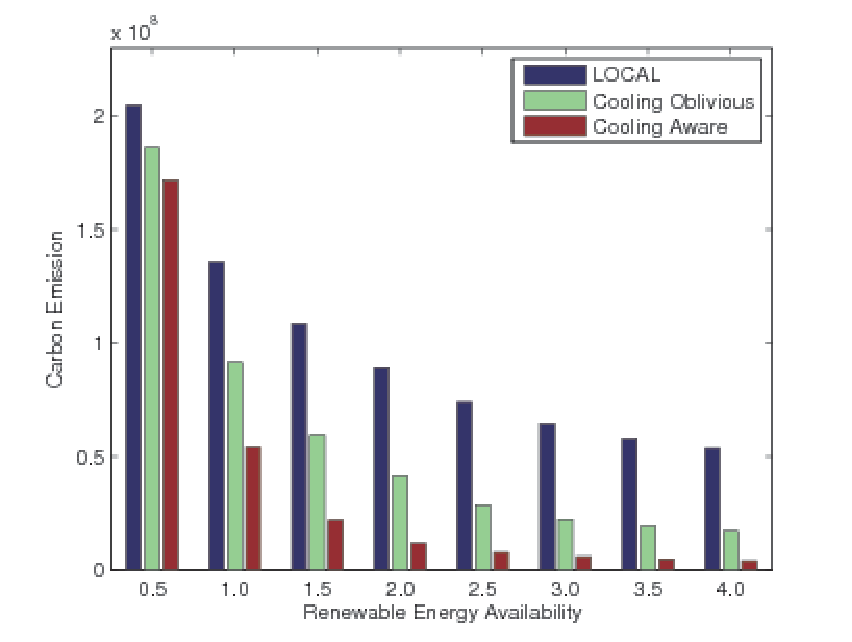
\epsfig{file=carbon_summer.pdf, height=2.2in, width=3.2in}
\caption{Comparison of carbon emission of Cooling-aware GLB, Cooling-oblivious GLB and LOCAL.}
\end{figure}

\end{frame}

\begin{frame}{}

\vspace{-3mm}
\begin{block}{\carbondioxide{} emission}
\vspace{-3mm}
$$\sum_{i \in \mathcal{N}} \eta_i \cdot (x_i(t) + c(x_i(t)) - r_i(t) - e_i(t))^+$$
Emissions rate $\eta_i$ per kW$\cdot{}$h varies across states based on energy-source composition.  %estimates available from \cite{carbon}.
\end{block}


%\begin{frame}{}
%\begin{block}{Storage ***** Eric, pls edit as you see fit *********}
%DC can store energy (batteries, supercapacitors, flywheels).

%Electricity storage at time $t$ is $0 \leq es_i(t) \leq ES_i$. 

%$ES_i$ = maximum storage capacity.  Storage rate is
%$$e_i(t) = \rho \cdot (es_i(t) - es_i(t+1))$$
%Positive $e_i(t)$ means discharging, negative charging. 

%Assume $\rho = 1$, charging or discharging efficiency is perfect.

%Energy cost with storage is
%\begin{equation}
%p_i \cdot (l(x_i(t)) + c(x_i(t)) - r_i(t) - e_i(t))^+
%\end{equation}
%\end{block}
%\end{frame}

\begin{frame}{GLB versus Storage}

\begin{figure}
\centering
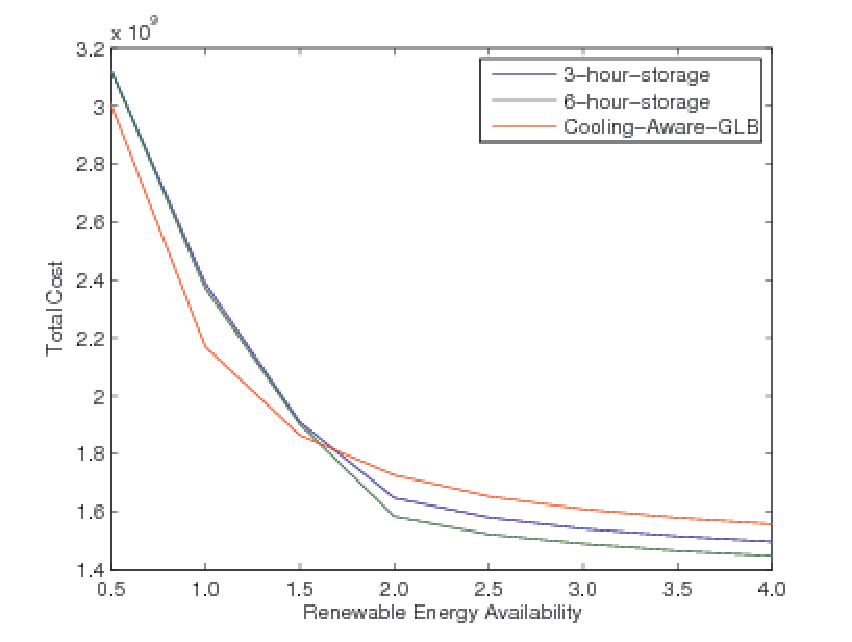
\epsfig{file=cost_storage.pdf, height=2.2in, width=3.2in}
\caption{Comparison of optimal costs of the storage model and the Cooling-aware GLB model.}
\end{figure}
\begin{figure}
\centering
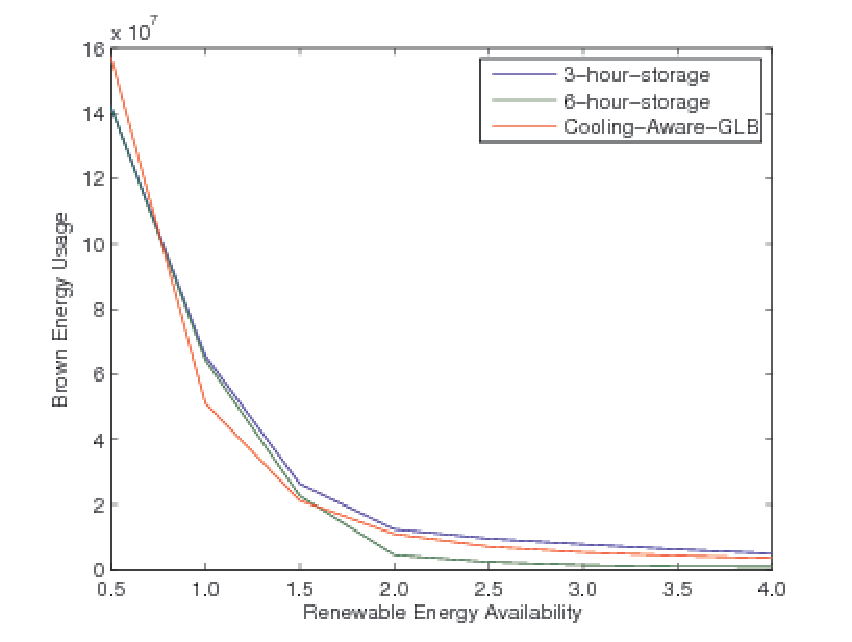
\epsfig{file=brown_storage.pdf, height=2.2in, width=3.2in}
\caption{Comparison of brown energy usage of the storage model and the Cooling-aware GLB model.}
\end{figure}
\end{frame}



\end{document}
